\chapter{Resultados Obtidos}

Para validar o sistema é preciso testar os requisitos: mecânicos, de custo, e de desempenho do aplicativo atuando em conjunto com a eletrônica. Então, foram realizados uma sequência de testes em campo. Além disso, a plataforma fora enviada para um astrofotógrafo e Engenheiro, convidado, que conduziu testes usando seu equipamento.\footnote{Relatório do Astrofotógrafo Ricardo Batista pode ser acessado neste link: LINK AQUI}

\section{Requisitos mecânicos}

Os objetivos mecânicos da plataforma foram alcançados com ressalvas. A plataforma montada totalizou 716g sem o \textit{Ball Head} da câmera, estando dentro da faixa de peso comparando com dispositivos similares no mercado. Ademais, a impressão 3D não se comportou como o esperado; somado a isso, existe um erro de inconsistência e vibração motivado por falha de fabricação na barra de elevação curva que deve ser analisado.


\subsection{Impressão 3D}
A engrenagem menor é o elo mais fraco no sistema de transmissão, que se deve pelo seu tamanho mais reduzido. A primeira versão da impressão 3D acabou sofrendo um rachamento por não suportar o torque do motor. Na Figura \ref{fig:engrenagem} é possível verificar que o rasgo se forma perpendicularmente com a tangente da engrenagem, evidenciando esse motivo de ruptura.

\begin{figure}[htb]
	\centering
	\caption{Engrenagem com rachamento em evidência}
	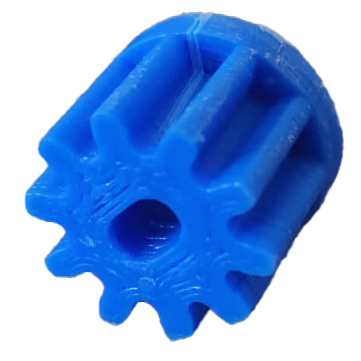
\includegraphics[width=0.25\linewidth]{figuras/resultados/engrenagem}
	\label{fig:engrenagem}
	\fonte{Autor.}
\end{figure}

Além disso, quando a engrenagem apresentou a rachadura, o peso do sistema totalizava mais de 2,5kg com o \textit{Ball-Head }Maxxi Grua somado à câmera CANNON 6D MARK II com uma lente 70-200mm. Contudo, este acontecimento não invalida o projeto pois ocorreu com um peso de rastreamento superior a meta proposta, e, por isso, recomenda-se cautela em situações onde o equipamento se aproxima ou ultrapassa a marca de 2,5kg de peso total.
 

\subsection{Eixo Curvado}
Além do problema com a engrenagem, o movimento de elevação da barra roscada se mostrou inconstante em certos pontos. Essa variação reflete a não idealidade da curvatura dessa barra. A Figura \ref{fig:validaçãoBarraRoscada} torna claro a discrepância entre como deveria ser, e como ficou. Esse erro de fabricação gerou inconsistência em certos pontos no funcionamento da plataforma, e eles serão demonstrados na próxima seção.

\begin{figure}[htb]
	\centering
	\caption{Erro de fabricação demarcado em vermelho, onde a barra apresenta uma curvatura que varia em relação ao desenho técnico}
	\includegraphics[width=0.8\linewidth]{figuras/resultados/validaçãoBarraRoscada}
	\label{fig:validaçãoBarraRoscada}
	\fonte{Autor.}
\end{figure}


\subsection{Análise de Consistência}
\label{sec:vibracao}

A velocidade e vibração da plataforma foram analisados por meio de um sensor acelerômetro instalado na base superior, como demonstra a Figura \ref{fig:sensorInstaladoPlataforma}. Com esse teste, foi possível comparar diferentes cenários de uso de elementos amortecedores no sistema e o seu impacto na consistência e vibração. Os dados foram obtidos em uma taxa de 100Hz, utilizando um Arduíno e comunicação Serial com um notebook que armazenava os dados \footnote{O sistema de captação de dados com o sensor está documentado neste repositório do Github: Link AQUI}. 

\begin{figure}[htb]
	\centering
	\caption{Sensor instalado na base superior}
	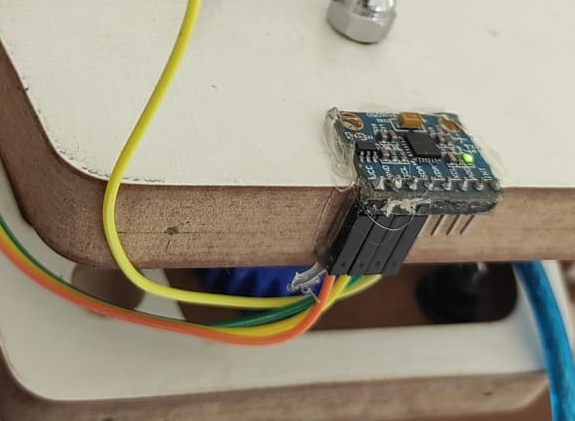
\includegraphics[width=0.35\linewidth]{figuras/resultados/sensorInstaladoPlataforma}
	\label{fig:sensorInstaladoPlataforma}
	\fonte{Autor.}
\end{figure}

Então, os dados obtidos no primeiro teste -- que constam na Figura \ref{fig:antes} --, demonstram que existia uma inconstância na velocidade angular do sistema, além de um excesso de vibração. Além disso, com os dados da Figura \ref{fig:depois}, confirmou-se que existe a necessidade de elementos para dissipar a vibração. Ressalta-se ainda que existem pontos de intensificação da vibração, e, pelo período temporal onde acontece, é possível inferir que são decorrentes do erro de fabricação do eixo curvado. 

\begin{figure}[!htb]
	\centering
	\caption{Primeiro teste do sistema}
	\includegraphics[width=0.9\linewidth]{figuras/resultados/antes}
	\label{fig:antes}
	\fonte{Autor.}
\end{figure}

\begin{figure}[!htb]
	\centering
	\caption{Teste do sistema com elementos amortecedores}
	\includegraphics[width=0.9\linewidth]{figuras/resultados/depois}
	\label{fig:depois}
	\fonte{Autor.}
\end{figure}

\section{Custo total do sistema}
O custo dos materiais e processos de fabricação estão descritos na tabela \ref{table:custo}\footnote{Alguns valores são aproximados pois foram doados pela Universidade}, com a qual pode se constar um total de 305 reais envolvendo materiais e fabricação de componentes. Comparando ao valor do NyxTech -- que possui uma construção e materiais similares, com um preço de US\$ 110 -- o EasyTracker conseguiu vencer a meta de custo.  

\begin{table}[!htb]
	\centering
	\caption{Descrição aproximada dos Custos do Sistema}
	\begin{tabular}{c|c}
	Item	&	Custo	\\\hline\hline
	MDF	15mm	&	R\$ 25,00		\\\hline
	Corte a Laser			&	R\$ 100,00		\\\hline
	PCB			&	R\$ 50,00		\\\hline
	Componentes Eletrônicos			&	R\$ 95,00		\\\hline
	Outros Materiais		&	R\$ 35,00		\\\hline\hline
	Total			&	R\$ 305,00		\\
	\end{tabular}
	\label{table:custo}
	\fonte{Autor.}
\end{table}


\section{Análise de desempenho do aplicativo}
O \textit{software} pode ser avaliado com relação ao uso e implementação das heurísticas de desenvolvimento, com relação ao desempenho em \textit{hardware} -- consumo de processamento e memória --, e ainda pode ser avaliado com \textit{feedbacks} dos usuários. 

\subsection{Interface Gráfica}
Quando à interface e recursos, é possível avaliar de forma qualitativa como as 10 Heurísticas de Nielsen foram utilizadas. Os status cruciais para funcionamento são todos visíveis: o \textit{status} \textit{bluetooth} do sistema é visível por meio do estado do botão de conexão na tela de visualização do perfil. Nas telas de alinhamento, se o sistema está alinhado, os ícones ficam esverdeados, caso contrário ficam avermelhados.

Além disso, as cores e os elementos de ícones são similares com o que os usuários estão acostumados, como os ícones nas telas de perfis de localização que fazem sentido para o contexto e são minimalistas. Além disso, as telas de alinhamento se assemelha a uma bolha de nível onde o acelerômetro é empregado. Na tela de alinhamento com o polo magnético, o sistema emula uma bússola. 

Nessas mesmas telas de alinhamento, os usuários podem controlar livremente o fluxo das telas de alinhamento. Dessa forma conseguem conferir alguma informação que possam ter ignorado, assim como podem navegar para telas de suporte. Não obstante, a consistência desses padrões nas telas de alinhamento também foi consolidado nas telas de perfis. As ações de criar, editar, e visualizar um perfil usam por base a mesma tela, facilitando para o usuário entender como utilizar o aplicativo. 

Além disso, a prevenção de erros é feita de forma ativa relembrando o usuário de, por exemplo, calibrar a bússola ao entrar na tela de alinhamento azimutal, ou também com um \textit{popup} para atualizar os dados de declinação magnética em localizações que foram armazenadas e não foram atualizadas por mais e 2 meses. A prevenção também ocorre nas entradas de dados:  onde o usuário precisa inserir valores de latitude e declinação, que devem ser valores decimais (Figura \ref{fig:gpsedit}). No entanto, eles podem ser escritos em graus, minutos e segundos, mas o usuário não vai conseguir inserir dessa forma, pois, o teclado numérico não permite essa formatação.

\begin{figure}[!htb]
	\centering
	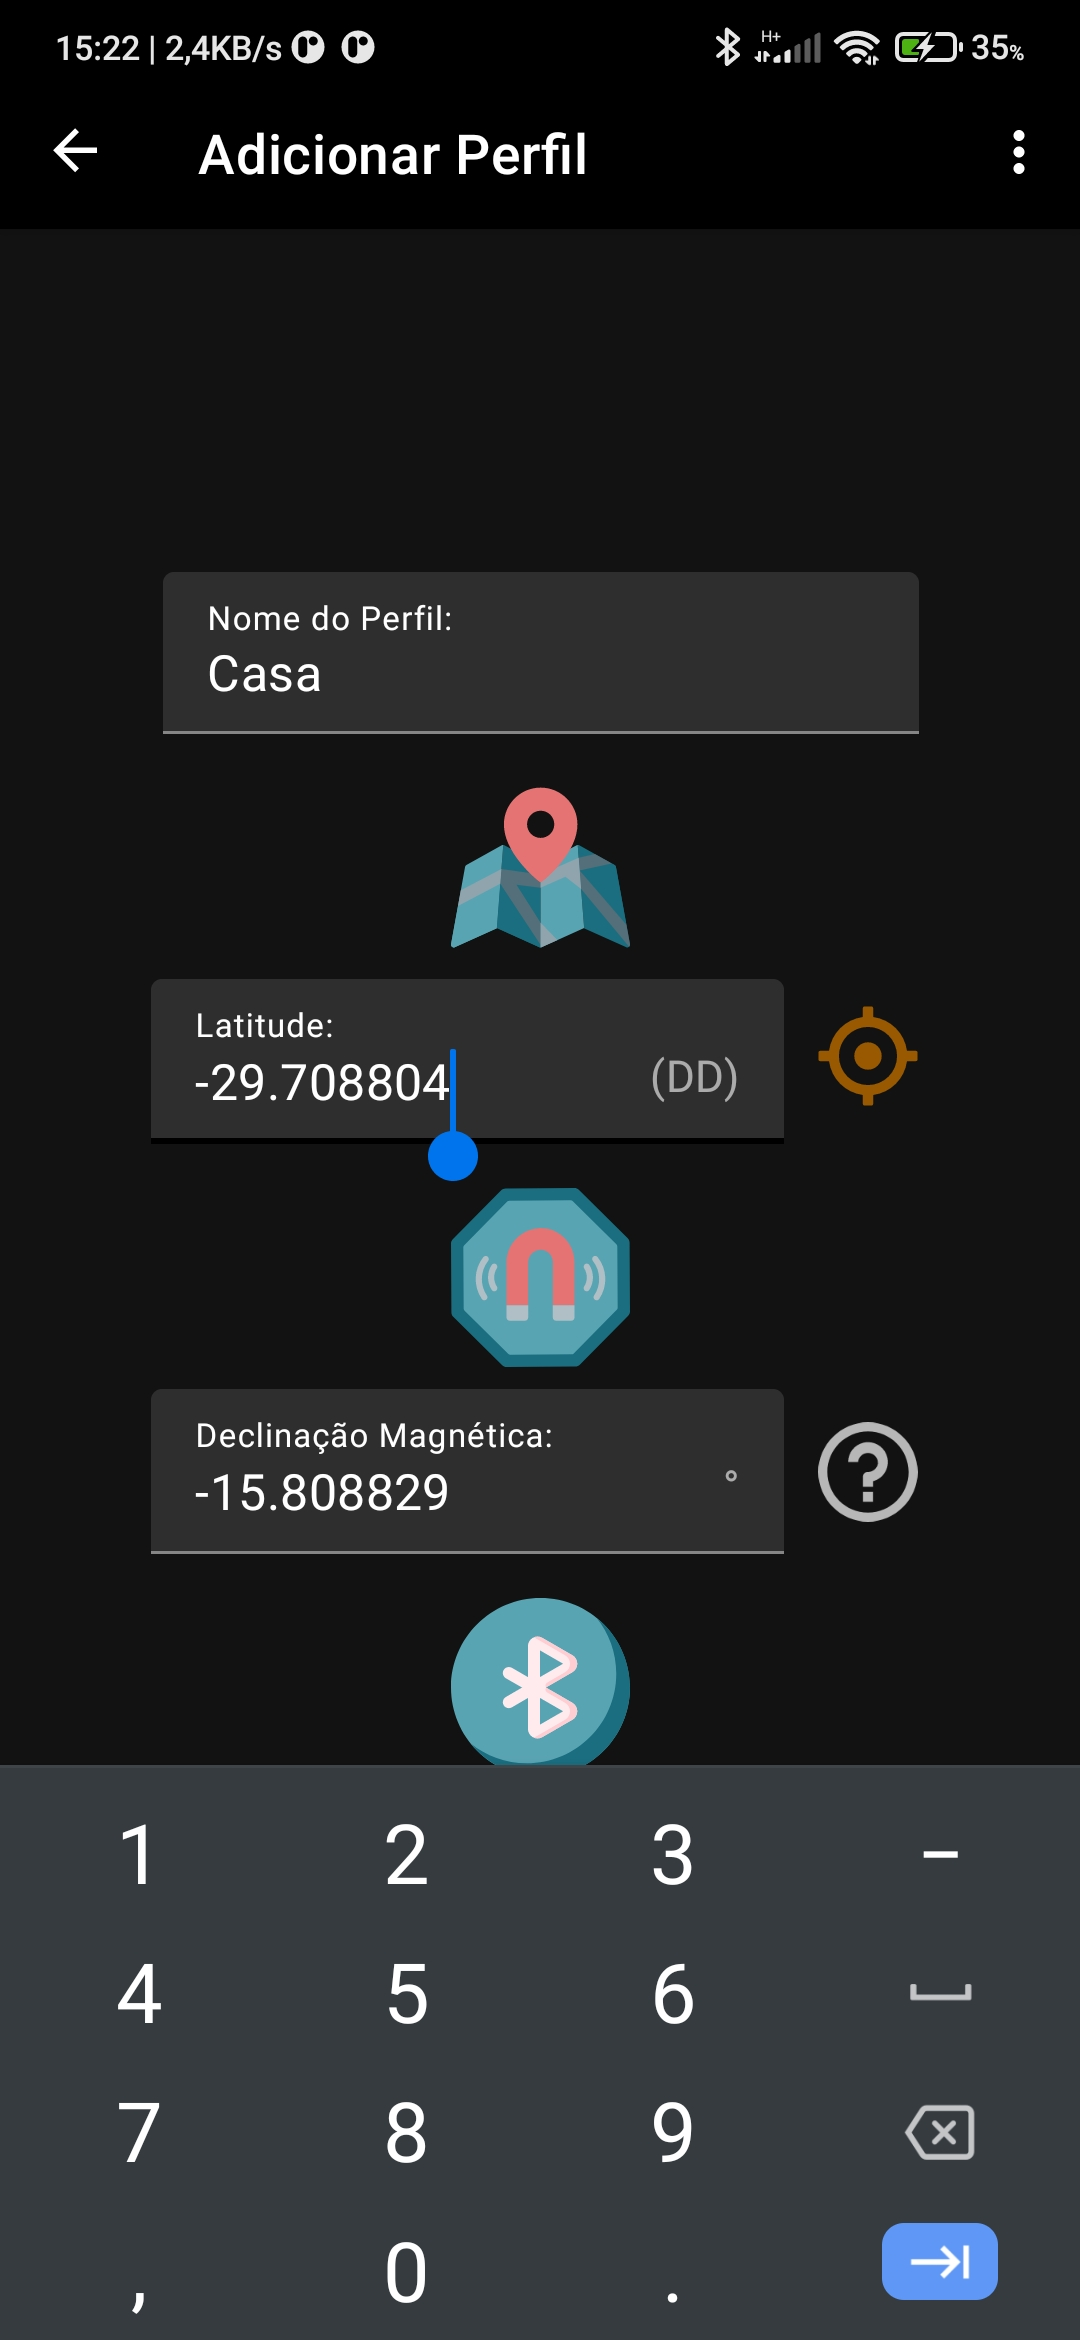
\includegraphics[width=0.3\linewidth]{figuras/resultados/gpsedit}
	\caption{Teclado só permite uso de vírgula e ponto, não permitindo aspas e sinal de grau $ (^\circ) $}
	\label{fig:gpsedit}
\end{figure} 

Dessa forma, o desenvolvimento da interface gráfica do aplicativo conseguiu atingir um estágio de desenvolvimento compatível com o estado da arte atual relativo a criação de aplicativos Android ou outros Softwares. As heurísticas foram respeitadas e a implementação é fluída, os itens estão dispostos respeitando uma hierarquia visual que está em conluio com a identidade do projeto e os recursos do Sistema Android. 

\subsection{Desempenho}
O aplicativo foi lançado na loja de aplicativos Android via Google Play Console. O Console de desenvolvedor realiza testes automáticos com alguns dispositivos e avalia o desempenho. Os resultados indicam que o aplicativo pode ter problemas de lentidão em hardwares mais antigos e com menor capacidade de memória e armazenamento; mas, ao mesmo tempo, não detectou nenhum problema em sistemas mais recentes (Figura \ref{fig:relatorioDesempenho}).

\begin{figure}[htb]
	\centering
	\caption{Resultados apresentados no Google Play Console}
	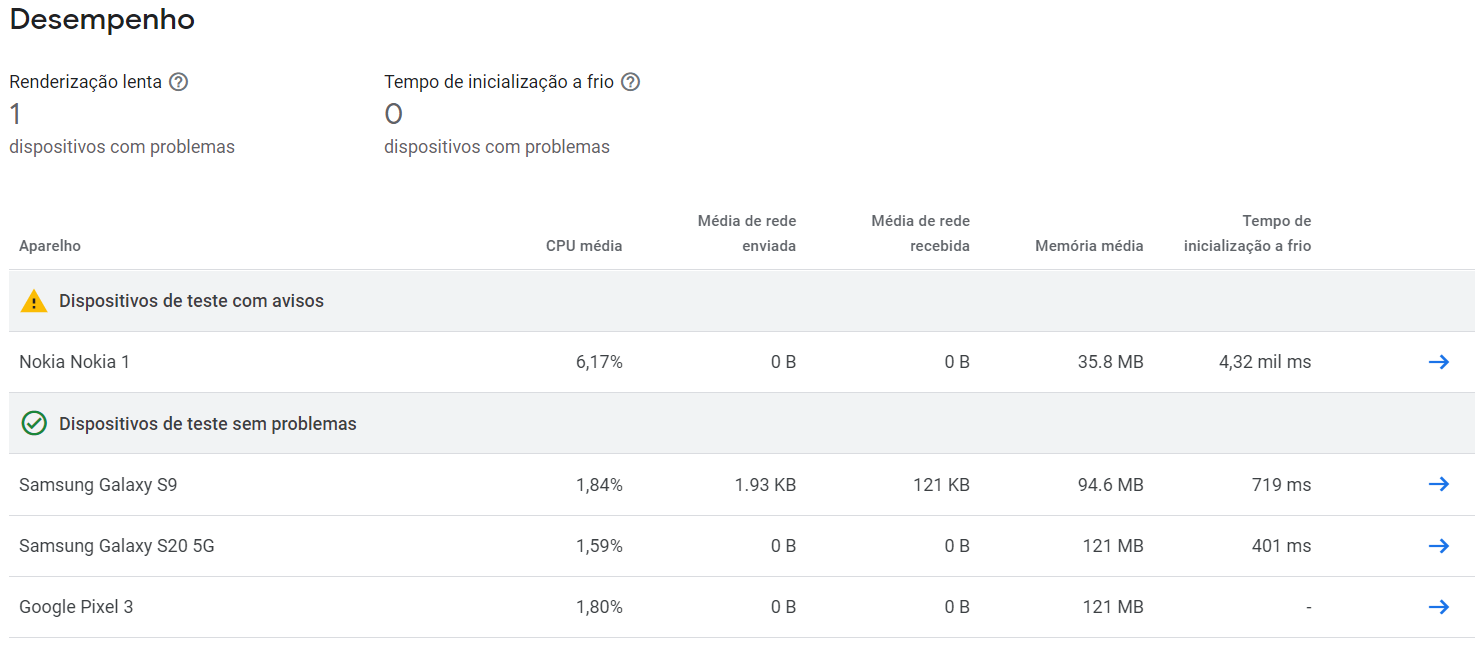
\includegraphics[width=\linewidth]{figuras/resultados/relatorioDesempenho}
	\label{fig:relatorioDesempenho}
	\fonte{Autor.}
\end{figure}

Considerando que o dispositivo com dificuldade no processamento é defasado, é razoável considerar que o aplicativo não trará problema para a maior parcela de dispositivos. 

\section{Comparativo Geral}
Os 3 pontos avaliados anteriormente listam eventuais problemas que afetaram a consistência do sistema e projeto como um todo. No entanto, é necessário verificar ainda se, apesar desses entraves, o projeto consegue cumprir com os objetivos gerais: se o método de alinhamento é tão confiável quanto os métodos tradicionais de luneta e laser; assim como se as especificações de erro estão dentro da margem comercial. Dessa maneira, dois erros podem ser avaliados: o erro inerente ao sistema mecânico, nomeado de erro periódico; e o erro relativo ao processo de alinhamento.


\subsection{Erro Periódico}

O erro periódico mensura a oscilação do sistema de transmissão, gerada por variações na montagem e encaixe dos componentes. O período desse erro é definido pelo tempo total levado para que o motor de passo realize 1 rotação. O erro é medido em arco-segundos (arcsec), que é uma unidade que irá avaliar o quanto uma estrela alternou sua posição pelo visor da câmera, em uma fração de graus, independente da lente utilizada. O teste que mensura esse erro é realizado apontando a câmera para qualquer alvo no céu, desalinhando o rastreador propositalmente, e realizando uma fotografia de longa exposição \cite{site:nyxtechFAQPeriodicError}. 

Então, apontou-se a câmera para Júpiter, utilizando a Câmera DSC-HX300, com comprimento focal em $ d = 192~mm $, e assim fora possível extrair a seguinte oscilação do posicionamento da estrela ao longo de 8 fotografias captadas em intervalos de 10s. Empilhando as imagens, têm-se o resultado da Figura \ref{fig:periodicErrorImage}. Usando um software editor de imagens, é possível desenhar sobre esses pontos uma forma de onda. O erro periódico é igual a distância de pico a pico medida em arc segundos. Essa distância é medida inicialmente em pixel, e posteriormente convertida para arcsec com as equações (\ref{eq:arc}) e (\ref{eq:erroperiodic}), sabendo que essa câmera tem um tamanho de pixel ($ px_s $) igual a  $ 1,19~um $ e sendo $ d_{AB} $ a distância em pixel pico a pico da onda. Esse procedimento foi realizado também com outros equipamentos, e com diferentes alvos, e a média de erro periódico calculado foi igual  $ 63~arcsec  $. Os resultados documentados podem ser conferidos no apêndice \ref{apendice:periodic}.


\begin{equation}
	ang_{Res}~(arcsec/px) = \dfrac{px_s~ (\mu m) * 206,3}{d~ (mm)}
	\label{eq:arc}
\end{equation}

\begin{equation}
	Erro_{periodico}~(arcsec) = d_{AB}~(px) \times ang_{Res} ~(arcsec/px)
	\label{eq:erroperiodic}
\end{equation}

\begin{figure}[htb]
	\centering
	\caption{Pontos obtidos com as 8 imagens sobrepostas, que foram captadas com intervalos de 10s}
	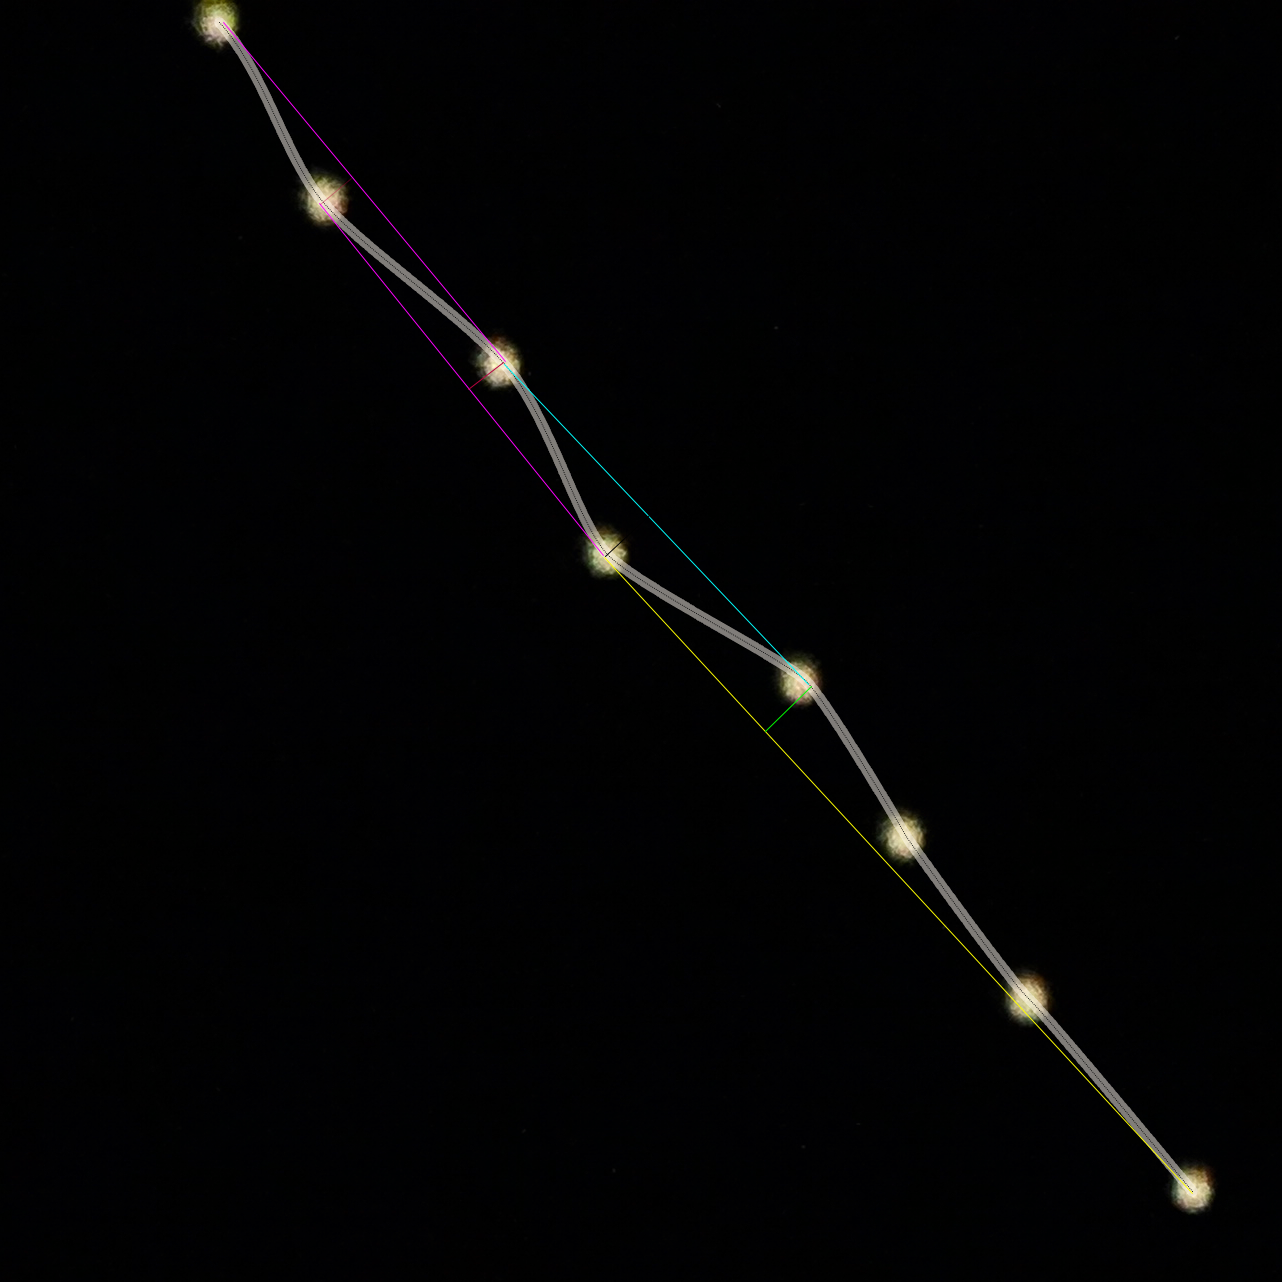
\includegraphics[width=.8\linewidth]{figuras/resultados/periodicErrorImage}
	\label{fig:periodicErrorImage}
	\fonte{Autor.}
\end{figure}


\subsection{Erro de Alinhamento}

Um alinhamento bem feito está diretamente relacionado ao tempo de exposição máximo de uma foto registrada com a câmera montada no EasyTracker. Segundo o convidado Ricardo Batista, em seu relatório, o iOptron SkyGuider Pró consegue proporcionar até 4 \textit{stops} extras de exposição, com um alinhamento pela luneta. Isso significa dizer que o tempo total de exposição que é possível atingir com rastreamento é de $ t_{max} = t_{atual} \times 2^{stop = 4} $; onde o $ t_{atual} $ é o tempo utilizado para fotografias sem rastreamento. 


Para determinar quantos "\textit{stops}" é possível atingir, é necessário avaliar o erro de rastreamento da plataforma ao longo de um período de tempo. Com base nesse erro, determina-se o tempo máximo de exposição para que a estrela não passe de um limite de tolerância especificado pela Regra NPF (seção \ref{sec:regraNPF}). Essa tolerância indica quantos pixeis uma estrela pode mover-se na captura da imagem, sem que isso seja um rastro indesejável. Assim, com o erro determinado, compara-se o tempo pela regra NPF e o tempo de rastreamento máximo estimado pelos valores empíricos; calculando quantos stops extras são possíveis de se obter com o alinhamento da plataforma.

Então, em diferentes condições e câmeras, foram realizadas diversas capturas, anotando o tempo de intervalo entre elas. Todas fotografias foram realizadas com o rastreador ligado e alinhado. Com elas, foi possível determinar quantos pixeis a estrela deslocou no período de tempo observado, obtendo, com isso, a velocidade angular de erro. Com a equação (\ref{eq:arc}) utilizada na seção anterior, determina-se a resolução angular da câmera, e pode-se então determinar quantos arcsec/s de erro acumula-se durante o rastreamento do EasyTracker.

Com a regra NPF, então, determina-se o tempo de exposição correto para que não haja rastro, $ tmax_{NPF} $. Sabendo a resolução angular da câmera e a velocidade angular da terra em arcsec/s calculado na equação (\ref{eq:arcsecTerra}), determina-se a tolerância do rastro de pixeis, $ NPF_{tol.} $,  com a regra NPF com a equação (\ref{eq:tolerancia}). 

\begin{equation}
	V_{terra} = \dfrac{360 \cdot 3600}{23\cdot3600+55\cdot60 + 4} = 15,04~arcsec/s
	\label{eq:arcsecTerra}
\end{equation}

\begin{equation}
	NPF_{tol.} = \dfrac{tmax_{NPF} ~\left[s\right]\cdot V_{terra}}{ang_{Res}~\left[arcsec/px\right]}~\left[px\right]
	\label{eq:tolerancia}
\end{equation}

Dessa maneira, calcula-se o tempo máximo, $ t_{max} $, de rastreamento com a equação (\ref{eq:tmax}) sabendo: o erro de rastreamento do sistema, $ V_{erro} $; a tolerância de pixeis $ NPF_{tol.} $; e a resolução angular da câmera, $ ang_{Res}~\left[arcsec/px\right] $. Esse resultado, quando comparado ao tempo dado pela regra NPF, determina quantos stops de exposição foi possível obter com o EasyTracker. 

\begin{equation}
	t_{max} = \dfrac{NPF_{tol.}\cdot ang_{Res} }{V_{erro}} \left[s\right]
	\label{eq:tmax}
\end{equation}

Nos testes mais recentes, possuindo prática com o equipamento, fora possível obter até $ 4,46 $ stops de exposição. O apêndice \ref{apendice:alignment} contém uma tabela registrando as medidas obtidas com cada captura realizada em testes. 

Os testes conduzidos pelo convidado também levaram à marca de 4 stops. Também foi possível verificar que o método do aplicativo é muito mais ágil quando comparado aos tradicionais, podendo ser realizado em até quatro minutos. Isso é quatro vezes mais rápido comparando com o tempo necessário para alinhamento realizado usando a luneta do iOptron SkyGuider Pro e executado por um profissional experiente. 